

\chapter[Adoção de Métodos Ágeis na Gestão de Demandas de Desenvolvimento de \textit{Software} em Organizações Públicas Brasileiras]{Adoção de Métodos Ágeis na Gestão de Demandas de Desenvolvimento de \textit{Software} em Organizações Públicas Brasileiras}

\section[Metodologias Ágeis de Desenvolvimento de \textit{Software}]{Metodologias Ágeis de Desenvolvimento de \textit{Software}}

Ao longo da evolução dos processos de Engenharia de \textit{Software}, a indústria se baseou nos métodos tradicionais de desenvolvimento de \textit{software}, que definiram por muitos anos os padrões para criação de \textit{software} nos meios acadêmico e empresarial. Porém, percebendo que a indústria apresentava um grande número de casos de fracasso, alguns líderes experientes adotaram modos de trabalho que se opunham aos principais conceitos das metodologias tradicionais. Aos poucos, foram percebendo que suas formas de trabalho, apesar de não seguirem os padrões no mercado, eram bastante eficientes   \cite{filho}. 

Em 2001, 17 líderes que estavam desenvolvendo projetos de formas diferentes aos padrões até então pregados pela indústria se reuniram em uma estação de ski em Utah para discutir seus trabalhos e experiências, no final da reunião, eles formaram um grupo intitulado de Aliança de Desenvolvimento Ágil e escreveram O Manifesto Ágil, o qual é constituído de princípios e valores que o grupo considerou determinantes para bons resultados no desenvolvido de \textit{software}. Com isso, os métodos de desenvolvimento de \textit{software} ágeis, em contraste com os métodos tradicionais dirigidos a planos, são baseados em quatro valores advindos do Manifesto Ágil, são eles \cite{manifesto}:
\begin{itemize}
\item Indivíduos e interações acima de processos e ferramentas;
\item \textit{Software} operante acima de documentações grandes e completas;
\item Colaboração do cliente acima de negociações contratuais;
\item Responder à mudanças acima de seguir um planejamento.
\end{itemize}

As declarações destes valores têm um formato fácil de se identificar. A primeira parte da sentença indica a preferência, enquanto a segunda parte da sentença indica algo que, embora importante, tem prioridade menor. Assim, a Aliança e o Manifesto Ágil, por exemplo, reconhecem a importância da documentação, processos e ferramentas, no entanto, reconhece também que, a interação entre indivíduos capacitados tem ainda maior importância.

Dessa maneira, uma documentação completa e de fácil entendimento não é ruim, porém, o foco primário deve estar na entrega de um  \textit{software} operante e na interação entre as pessoas. Nesse contexto, a negociação contratual é um prática insuficiente, pois, os contratos podem apresentar condições de fronteiras nas quais os envolvidos podem trabalhar, mas somente com a contínua colaboração entre cliente e equipe é que se consegue entender e entregar o que o cliente realmente deseja \cite{jim}. Assim, um plano detalhado, elaborado no início de um projeto de desenvolvimento de \textit{software} pode acarretar riscos, caso ele impeça que mudanças ocorram. Esse ponto pode ser conflitante com a necessidade de planejamento e o princípio da impessoalidade, inerentes às contratações públicas. No entanto, é possível alinhar a utilização desses valores ágeis aos preceitos legais, mediante a atenção a certas cautelas \cite{TCU:2013}.

Os valores ágeis estão relacionados aos doze princípios também advindos do Manifesto Ágil, são eles \cite{manifesto}:
\begin{itemize}
\item Satisfaça o cliente por meio da entrega rápida e contínua de  \textit{software} que traga valor;
\item Mudanças nos requisitos são aceitas, mesmo em estágios avançados de desenvolvimento;
\item  \textit{Software} funcionando é entregue frequentemente em curtos períodos de tempo;
\item As pessoas relacionadas ao negócio e os desenvolvedores devem trabalhar em conjunto diariamente;
\item Construa projetos formados por indivíduos motivados, forneça o ambiente e suporte necessário e confie que eles realizarão o trabalho;
\item O modo mais eficiente e eficaz de transmitir informações dentro e fora do time de desenvolvimento é a comunicação face a face;
\item A principal medida de progresso é o  \textit{software} funcionando;
\item Processos ágeis promovem o desenvolvimento em ritmo sustentável, onde os envolvidos devem ser capazes de manter o ritmo constante;
\item Cuidar continuamente da excelência técnica e do bom \textit{design} ajuda a aprimorar a agilidade;
\item Simplicidade – a arte de maximizar a quantidade de trabalho não necessário – é essencial;
\item Os melhores requisitos, arquiteturas e \textit{design} surgem de equipes auto gerenciadas;
\item Em intervalos regulares, a equipe reflete sobre como se tornar mais eficiente, refinando e ajustando seu comportamento apropriadamente.
\end{itemize}

A partir de então, diversas práticas que já eram aplicadas a alguns projetos se transformaram em métodos de desenvolvimento de  \textit{software}, baseadas nos princípios e valores ágeis, como exemplo o Scrum e o \textit{Extreme Programming} (XP). A abordagem ágil compartilha de arcabouço teórico semelhante ao utilizado para definição dos conceitos Lean, além de sua adaptação ao contexto do desenvolvimento de  \textit{software}. Pode-se abservar, por exemplo, que ambas dão ênfase à satisfação do cliente e entrega rápida do produto.

\subsection[Scrum]{Scrum}

O Scrum é uma metodologia que começou a ser desenvolvida na década de 90 \cite{ken}. Ele se concentra nos aspectos gerenciais do processo de desenvolvimento de \textit{software}. É uma abordagem que favorece o empoderamento de equipes auto organizáveis e integração com outras metodologias que foquem em práticas relacionadas à programação, como o XP.

O Scrum caracteriza-se por ser um processo empírico e adaptativo propondo iterações de curta duração (as chamadas \textit{Sprints}) com reuniões de acompanhamento diárias (chamadas de \textit{Daily Meeting}) realizadas de pé, as quais permitem a identificação antecipada de eventuais problemas e a visibilidade do que está sendo feito por todos. A Figura (9) apresenta o ciclo de vida do processo Scrum.

\begin{figure}[h]
	\centering
		\label{fig01}
			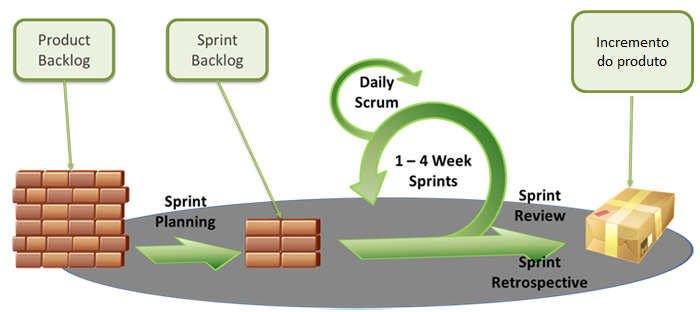
\includegraphics[scale=0.8]{figuras/scrum.png}
		\caption{Framework Scrum}
\end{figure}

No processo Scrum são definidos três papéis: Scrum \textit{Master}, aquele que deve ensinar a utilizar o Scrum, acompanhar o desenvolvimento e resolver impedimentos; \textit{Product Owner}, aquele que deve garantir que o produto atenda as necessidades do cliente ou patrocinador do projeto e deve priorizar as funcionalidades que agreguem mais valor ao cliente; e a Equipe de Desenvolvimento   \cite{jeff}.

Os requisitos do produto são expressos por meio das histórias de usuário, que em seu conjunto compõêm o artefato conhecido como (\textit{Product Backlog}. No início de cada \textit{Sprint} é feita uma reunião de planejamento (\textit{Sprint Planning}) na qual uma estimativa e a meta da \textit{Sprint} são definidas e algumas histórias de usuário (\textit{User Stories}) que estão no \textit{Backlog} do Produto são selecionadas e transformadas em tarefas do \textit{Backlog da Sprint}, as quais devem ser desenvolvidas para atingir a meta da \textit{Sprint}. Depois do planejamento, a equipe começa um ciclo de desenvolvimento do produto, que pode durar de uma a quatro semanas. Durante cada \textit{Sprint}, o \textit{Scrum Master} assegura que as histórias de usuário selecionadas não mudarão, permitindo que a equipe fique concentrada em seu objetivo. O \textit{Product Owner} acompanha o desenvolvimento e esclarece eventuais dúvidas. O \textit{Product Owner} só pode interferir no desenvolvimento da \textit{Sprint} se uma mudança de negócio afetar os requisitos do produto que está sendo desenvolvido  \cite{jeff}.

Quando uma \textit{Sprint} é finalizada, a equipe de desenvolvimento apresenta o trabalho feito na reunião de revisão da \textit{Sprint} (\textit{Sprint Review}). O \textit{Product Owner} faz testes e verifica se a meta foi realmente atingida. Ainda, após a entrega, a equipe realiza uma reunião de retrospectiva (\textit{Sprint Retrospective}) para analisar seu trabalho e oportunidades de melhoria para a próximo ciclo de produção.   \cite{jeff}. 

\section[Kanban, Scrum e o Pensamento Lean ]{Kanban, Scrum e o Pensamento Lean }

Scrum e Kanban são ferramentas de processo que, em certa medida, ajuda toda a equipe a trabalhar de maneira mais eficaz, por meio de instruções do que deve ser feito. Como qualquer ferramenta, Scrum e Kanban não atendem completamente a todas as situações. Eles não dizem absolutamente tudo que precisa ser feito, mas sim oferecem algumas restrições e orientações. Por exemplo, o Scrum restringe um tempo fixo para cada iteração e que as equipes devem ser multifuncionais, enquanto que o Kanban restringe a utilização de quadros visíveis e a limitar o tamanho da quantidade de trabalho a ser desenvolvido em um mesmo período de tempo. A utilização de ferramentas ajuda a ter sucesso, mas não garante por si só o sucesso. Tanto Scrum quanto Kanban são empíricos no sentido em que se espera que as pessoas experimentem o processo e o personalize segundo às necessidades da organização e do próprio time.

Scrum e Kanban são sistemas puxados (\textit{pull}), que correspondem ao princípio de gestão de inventário de \textit{Just In Time} (JIT) do Lean. Isso significa que a equipe escolhe quando e quanto de trabalho irá se comprometer para então “puxar” o trabalho quando estão prontos para começar, ao invés de ter que empurrar o trabalho de algum lugar. Scrum e Kanban são baseados em otimização empírica e continua do processo, que corresponde ao princípio de Kaizen do Lean.

Um modo de comparar essas duas ferramentas é analisando a quantidade de regras que elas oferecem. Quanto mais prescritivo for um processo, mais regras estão disponíveis para seguir. A idéia passa pelo entendimento de que não seria necessário muito esforço intelectual já que as regras já estão detalhadas. Quanto mais adaptativo um processo menos regras estão definidas para serem seguidas, ou seja, pode-se fazer qualquer coisa. Evidentemente, os dois extremos desta escala não é bom   \cite{kniberg2009}. 

Os métodos ágeis são por vezes chamados de métodos “leves” por serem menos prescritivos que os métodos tradicionais devido à quantidade de atividades, papéis e artefatos definidos. Scrum e Kanban são ambos adaptativos, mas ao realizar uma comparação entre as duas ferramentas, Scrum pode ser considerado mais prescritivo que o Kanban, pois existem mais restrições. Por exemplo, o Scrum prescreve um quadro de tarefas com as raias fixas, \textit{TO DO}, \textit{DOING} e \textit{DONE}, além do uso de iterações curtas. Já o Kanban não. O segredo está em não se limitar a uma única ferramenta. As ferramentas mais adaptativas podem ser combinadas de forma a trazerem mais benefícios para a organização. Na Figura (10) é apresentada uma escala comparativa em alguns métodos.

\begin{figure}[H]
		\centering
		\label{fig02}
			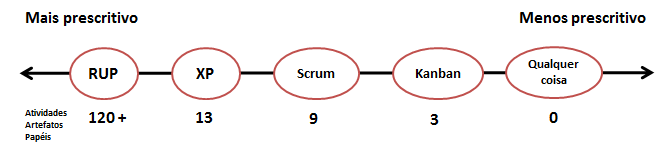
\includegraphics[scale=0.7]{figuras/prescritivo.png}
		\caption{Comparação entre métodos segundo segundo suas características prescritivas \cite{kniberg2009}}
\end{figure}

A despeito das considerações apresentadas e considerando que tanto o Scrum quanto o Kanban promovem um fluxo de trabalho contínuo e rápido. Porém, cabe ressaltar algumas diferenças observadas:

\subsection[Cadência]{Cadência}

No Scrum há uma única cadência de tempo, fixo, que combina quatro principais atividades: o planejamento, o desenvolvimento, a entrega do algo funcional e a melhoria. Uma cadência única diz respeito ao fato de manter as iterações com o mesmo tempo fixo durante um período de tempo realizando as mesmas atividades principais. Já no Kanban, não há esta prescrição de duração fixa de iterações, pode-se escolher uma periodicidade regular para realizar determinadas atividades ou pode-se escolher entregar sempre que tiver algo útil e funcional, ou seja, cadências distintas  \cite{kniberg2009}. 

\subsection[Limitação do WIP]{Limitação do WIP}

No Scrum, o \textit{Sprint Backlog} mosta quais são as tarefas a serem executadas durante a iteração atual. Geralmente, o \textit{Sprint Backlog} é representado no quadro Scrum ou quadro de tarefas. No Kanban, também existe o quadro de tarefas com propósito semelhante ao quadro utilizado no Scrum. Em ambos há o controle das tarefas ao longo do fluxo de trabalho. As colunas de ambos os quadros podem ser determinadas a gosto. A única coisa que torna um quadro diferente do outro é que no Kanban o trabalho em progresso (WIP), na raia “em progresso” ou nas demais colunas, é limitado explicitamente, enquanto no Scrum o limite explícito é apenas no tamanho das iterações (Fig. 11). 

\begin{figure}[H]
		\centering
		\label{fig03}
			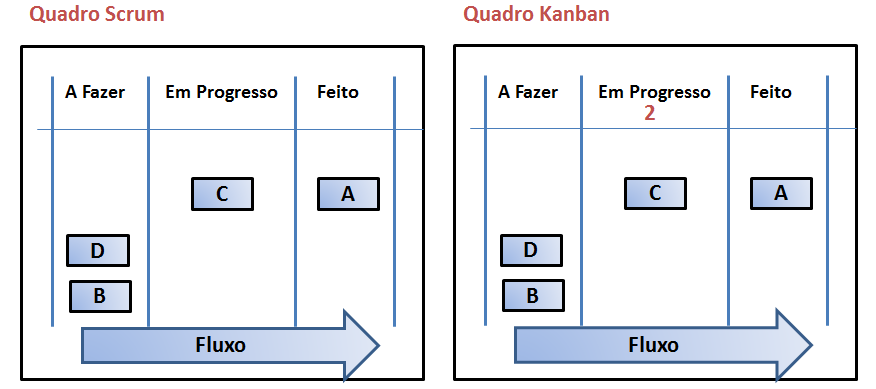
\includegraphics[scale=0.7]{figuras/quadros.png}
		\caption{Quadro Scrum x Quadro Kanban  \cite{kniberg2009}}
\end{figure}

Por vezes, uma equipe Scrum limita intuitivamente a quantidade de trabalho em progresso, evitando colocar mais atividades na coluna “em progresso” sem antes retirar as que lá estão. Quando uma equipe Scrum decide de fato limitar o WIP, então ela estará utilizando o quadro Kanban. Geralmente, as equipes Scrum medem sua velocidade (quantos pontos conseguem realizar em um determinado tempo) e com isso conseguem limitar a quantidade de trabalho em progresso.

Outra característica interessante que diferencia os dois quadros é que as tarefas no quadro do Scrum são movidas durante a iteração de forma que ao final espera-se que todas estejam na última coluna e o restante das colunas fique limpo, enquanto no quadro do Kanban sempre que uma tarefa é movida de coluna uma nova entra em seu lugar, sempre tendo tarefas em todas as colunas  \cite{kniberg2009}.

\subsection[Equipe de Trabalho]{Equipe de Trabalho}

Um quadro de tarefas no Scrum pertence a exatamente uma equipe Scrum. Uma equipe Scrum é multifuncional e tem papéis definidos, e esta contém todas as habilidades necessárias para completar todos os itens contidos na iteração. Um quadro de Scrum é geralmente visível a qualquer pessoa que esteja interessada, mas somente aqueles que fazem parte da equipe Scrum podem editá-lo – é a sua ferramenta para gerenciar o seu compromisso para esta iteração. Em Kanban, equipes multifuncionais são opcionais, e o quadro de atividades não precisa pertencer exclusivamente a uma única equipe. Um quadro de atividades está relacionado a um fluxo de trabalho, não necessariamente a uma equipe  \cite{kniberg2009}.

\section[Contratação Ágil nas Organizações Públicas Brasileiras]{Contratação Ágil nas Organizações Públicas Brasileiras}

\subsection[Iniciativas de Adoção de Métodos Ágeis no Governo]{Iniciativas de Adoção de Métodos Ágeis no Governo}

As metodologias ágeis começaram a ganhar espaço no início da década de 2000, regidas pelo Manifesto Ágil, e desde então vêm ganhando crescente popularidade. No cenário mundial, elas já são metodologias bastante difundidas entre diversos setores. Porém, no mercado nacional, essas metodologias são mais conhecidas e implementadas em empresas privadas. Atualmente, diversas organizações públicas brasileiras estão iniciando investimentos em adotação de contratações de fornecedores de \textit{software} utilizando métodos ágeis e, portanto, estão começando a difundir tais métodos também no setor público \cite{RTMAC}. 

Recentemente, o Tribunal de Contas da União publicou o Acórdão nº 2314/2013 o qual contém um relatório de levantamento elaborado pela Secretaria de Fiscalização de Tecnologia da Informação (SEFTI) cujo objetivo foi conhecer as bases teóricas do processo de desenvolvimento de \textit{software} com metodologia ágil, além de conhecer experiências práticas de contratação realizadas por instituições públicas federais. As instituições analisadas foram Banco Central do Brasil (BACEN), Instituto do Patrimônio Histórico e Artístico Nacional (IPHAN), Instituto Nacional de Estudos e Pesquisas Educacionais Anísio Texeira (INEP), Tribunal Superior do Trabalho (TST) e Supremo Tribunal Federal (STF). A seguir será relatada de forma resumida a experiência de cada instituição com o uso de metodologias ágeis em contratações de fornecedores de \textit{software} de acordo com o que foi apresentado no Acórdão nº 2314/2013 \cite{TCU:2013}.

O TST publicou seu primeiro edital para contratação de horas de serviço técnico para desenvolvimento e sustentação de sistemas em 2012. Antes disso, o órgão adquiriu uma experiência interna de desenvolvimento de \textit{software} utilizando o Scrum. A principal característica do edital publicado pelo TST foi: cada \textit{sprint} pode agrupar manutenções de sistemas diferentes e a equipe provavelmente terá que interagir com mais de um \textit{Product Owner}, pois este papel poderá ser representado por mais de uma pessoa. De acordo com o Acórdão nº 2314/2013, supracitado, não foi possível analisar a gestão contratual deste órgão, pois no momento da visita não havia ordem de serviço emitida nesse contrato.

O BACEN também publicou seu primeiro edital para contratação de serviço técnico de TI para desenvolvimento, documentação e manutenção de sistemas em 2012. Antes disso, o órgão já tinha uma experiência interna de desenvolvimento de \textit{software} utilizando métodos ágeis. Os serviços de desenvolvimento e manutenção seguem o Processo de Desenvolvimento de \textit{Software} Ágil (PDS-AGIL) definido pelo BACEN. Esse processo é baseado nas metodologias Scrum e XP, porém, por ser um processo de desenvolvimento desenhado para o uso interno, ele não deixa muito claro quais seriam as atividades específicas de contratação. 

O IPHAN teve sua primeira experiência com métodos ágeis no seu edital que foi publicado em 2011. Os serviços de contratação devem ser executados de acordo com a Metodologia IPHAN de Gestão de Demandas de Desenvolvimento Ágil de \textit{Software} (MIDAS) definida pelo órgão. A forma de execução dos serviços prevê o desenvolvimento do projeto em ciclos e cerimônias bem definidas baseado no Scrum. Esta instituição foi escolhida para estudo de caso deste trabalho e mais detalhes sobre a metodologia de gestão de demanda utilizada serão apresentados na próxima seção. 

O INEP teve seu primeiro edital com métodos ágeis de contratação de fábrica de \textit{software} para prestação de serviços técnicos de TI em 2011, o qual deveria ser executado segundo a orientação da Metodologia de Desenvolvimento de Sistemas (MGDS) definida pelo INEP, que é baseada em XP e Scrum. O órgão já está no seu segundo contrato utilizando métodos ágeis. A primeira contratação fracassou porque a equipe era composta basicamente de analistas juniores e eles não tinham conhecimento em desenvolvimento de sistemas utilizando métodos ágeis. Com isso, houve uma troca de empresas e a segunda contratação, após o período de adaptação, atendeu o esperado.

O STF inicialmente implantou o desenvolvimento de sistemas utilizando metodologia ágil, baseada no Scrum, em suas equipes internas. O seu primeiro edital para contratação de empresa para prestação de serviços de desenvolvimento ágil de soluções de \textit{software} foi publicado em 2012. A forma de execução dos serviços também é baseada no Scrum. Mais informações sobre a contratação não foram possíveis, pois no momento da visita da equipe de fiscalização o órgão não havia iniciado ainda a execução do contrato. 

De forma geral, o SEFTI analisou o trabalho desenvolvido nas instituições de acordo com três categorias: métrica utilizada, gestão das demandas e execução dos serviços e níveis de serviços estabelecidos. Quanto a métrica utilizada, a maioria das instuições analisadas utiliza como principal métrica o Pontos por Função, com exceção do TST que utiliza a métrica Horas de Serviço Técnico. 

Quanto à forma de gestão de demandas, a maior parte do instrumento convocatório das instituições é semelhante. A demanda para construção do produto é precedida pelo planejamento do produto, o qual pode ser feito apenas pela instituição contratante ou em conjunto com a empresa contratada. Além do planejamento do produto em si, algumas instituições também fazem o planejamento das funcionalidades que serão implementadas no próximo ciclo, iteração ou \textit{sprint}, atividade preceituada no Scrum. Estas instituições emitem uma ordem de serviço por ciclo, iteração ou \textit{sprint}, ou por \textit{release} de \textit{software}, sendo mais comum o primeiro caso. 

Quanto à aceitação do produto entregue pela contratada, embora no Scrum seja preceituado que ocorra na reunião de revisão da \textit{sprint}, essa prática não foi executada nos contratos estudados. Isso de deveu a força do normativo, como disciplinado no art. 73 da Lei nº 8.666/1993. Nessa ocasião, algumas instituições apenas verificavam se os artefatos exigidos foram entregues, caracterizando o recebimento provisório. 

Acerca da forma de pagamento da contratada, algumas instituições remuneram os serviços de planejamento, quando realizados, enquanto outras remuneram apenas os serviços de construção do \textit{software}. A entrega adiantada e contínua de \textit{software}, conforme postulado nos princípios dos métodos ágeis, foi observada em algumas das instituições. Para alcançar esse objetivo, elas paralelizam as atividades de preparação, execução e homologação, ou seja, em um dado período de tempo, enquanto a empresa contratada executa a construção do \textit{software} em um ciclo, a contratante prepara os itens do \textit{backlog} do produto \cite{TCU:2013}. 

Quanto à execução dos serviços e níveis de serviço estabelecidos observou-se que quase todas as instituições instituíram vários níveis de serviço a serem atendidos pela contratada. Em suma, o não atendimento a critérios mínimos aceitáveis implica a redução do valor a ser pago à contratada. Dos níveis de serviço analisados, verificou-se a preocupação quase comum das contratantes com o prazo para o cumprimento das iterações, ciclos ou \textit{sprints}, e com a qualidade dos produtos entregues  \cite{TCU:2013}.

\subsection[Desafios]{Desafios}

Algumas peculiaridades da Administração Pública e o seu arcabouço jurídico obrigatório (Lei nº 8.666/90, Instrução Normativa 04/2010 SLTI.MPOG e acórdãos do TCU) dificultam a adesão de instituições pública aos princípios Ágeis, principalmente em relação à contratação/terceirização de empresas prestadoras de serviços de desenvolvimento de \textit{software}.

Ordens de Serviços, Mensuração do Produto em Pontos por Função ou Horas de Serviços Técnicos, Termo de Recebimento Provisório e Termo Definitivo, Homologações Técnicas e Negociais, Atestes e Notas Fiscais são alguns dos documentos mínimos exigidos pela legislação que o Gestor Público e a Empresa Contratada terão que produzir independentemente se a metodologia adotada é ágil ou não. Somam-se ainda todos os documentos exigidos em cláusulas contratuais. 

Como isso, o excesso de documentação poderia ser inadequado aos valores ágeis de \textit{software} funcionando mais que documentação abrangente e responder a mudanças mais que seguir um plano. Ao mesmo tempo, a falta das principais documentações exigidas pode ferir o princípio de eficiência da Administração Pública Federal (APF) e, ainda, se não seguir de forma alguma o que foi  planejado, pode-se ferir também os princípios de planejamento e economicidade da APF. \cite{ruas}

Outro ponto relevante é a relação com equipe de desenvolvimento terceirizada. Em uma equipe externa (terceirizada), o Gestor Público não pode, por lei, interferir na conduta das pessoas contratadas, exceto via o Preposto, pois poderia ferir o princípio de impessoalidade da APF.

Na busca pela compatibilização entre o uso de métodos ágeis e adequação a legislação pertinente, algumas alternativas tem sido adotadas por instituições públicas, em suas iniciativas recentes, no uso de métodos ágeis. São elas: entrega de artefatos de documentação associados ao \textit{software} produzido a cada iteração; relação contratual prevalece sobre a possível colaboração entre as partes; escopo fixo dentro das iterações e níveis de serviços vinculados à qualidade do produto   \cite{ruas}. 

Com essas alternativas, alguns dos riscos inerentes são mitigados e não há o afastamento da legislação aplicável e ao mesmo tempo estão encaminhadas na direção dos valores e princípios ágeis. 

\section[Considerações Finais do Capítulo]{Considerações Finais do Capítulo}

A adoção de metodologias ágeis é um tema que vem ganhando destaque nos últimos
anos nas organizações públicas brasileiras, e, particularmente, dentro das contratações de fornecedores de desenvolvimento de software. Neste contexto, tem-se observado é necessário
adaptar os princípios e as práticas definidas nessa metodologia pra que elas se alinhem, também, aos
aos princípios e exigências legais da Administração Pública Federal. No próximo capítulo será apresentado o projeto do estudo de caso desse trabalho que tem como objeto de estudo a solução construída por uma organização pública brasileira que alinhou os princípios e as ferramentas ágeis com as exigências legais existentes na gestão de contratos de fornecedores de desenvolvimento de software.